\PassOptionsToPackage{table, dvipsnames}{xcolor}
\documentclass[a4paper,oneside,12pt]{toptesi}
\usepackage[T1]{fontenc}
\usepackage[utf8]{inputenc}
\usepackage[italian]{babel}
\usepackage{natbib} 
\bibliographystyle{plain}
\usepackage{graphicx}
\usepackage{tikz}
\usetikzlibrary{positioning}
\usepackage{pgfplots}
\usepackage[newfloat]{minted}
\usepackage[font=small,skip=1pt]{caption}
\usepackage{minted}
\usepackage{subcaption}
\pgfplotsset{compat=1.18}
\usepackage{lscape}
\usepackage{adjustbox}
\usepackage{graphicx}
\usepackage{wrapfig}
\usepackage{microtype}
\usepackage{tocloft}
\usepackage{xcolor}
\usepackage{hyperref}

\sloppy

\SetupFloatingEnvironment{listing}{name=Codice}


\usepackage{minted}
\usemintedstyle{monokai}
\definecolor{bg}{RGB}{40, 44, 52}



% ===== Define abstract environment =====
\newcommand{\prefacename}{Preface}
\newenvironment{preface}{
    \vspace*{\stretch{1}}
    {\noindent \bfseries \Huge \prefacename}
    \begin{center}
        % \phantomsection \addcontentsline{toc}{chapter}{\prefacename} % enable this if you want to put the preface in the table of contents
        \thispagestyle{plain}
    \end{center}%
}
{\vspace*{\stretch{1}}}


\newcommand{\walter}[1]{\textcolor{red}{{\bf [Walter: }{#1}{\bf ]}}}
\newcommand{\blueunderline}[1]{\textcolor{blue}{\uline{#1}}}

\usepackage{hyperref}

\hypersetup{
    colorlinks = true,
    allcolors=black
}

%%% workaround for listing
% save the current meaning of \listing
\let\savedlisting\listing
% at the right spot, restore the meaning
\AtBeginDocument{\let\listing\savedlisting}
%%% end of workaround


\def\dept{Dipartimento di Informatica}
\def\course{Corso di Laurea in Informatica}
\def\title{Guida utente dell'applicativo realizzato}
\def\author{Alessandro Carella}
\def\beforeprof{Professore}
\def\prof{Prof. Stefano Ferilli\newline\newline Prof. Berardina Nadja De Carolis}
\def\beforeRelatore {Relatrice}
\def\beforetitle{Tesi di Laurea in}
\def\subject{Informatica}
\def\annoacc{2022 - 2023}
\def\beforecandidate{Laureando}
\def\beforeannoacc{Anno Accademico}

\makeatletter
\def\cleardoublepage{\clearpage\if@twoside \ifodd\c@page\else
    \hbox{}
    \vspace*{\fill}
    \vspace{\fill}
    \thispagestyle{empty}
    \newpage
    \if@twocolumn\hbox{}\newpage\fi\fi\fi}
\makeatother


\begin{document}

%\maketitle


\begin{titlepage}
	\begin{tikzpicture}[remember picture,overlay]
		\centering
			\node[yshift=-6 cm] (logo) at (current page.north) {
\includegraphics[width=0.35\linewidth]{images/logo uniba.png}};
			\node[text width=50em,yshift=0.25cm, align = center, below = of logo](uniba){\bfseries \Large Università degli Studi di Bari Aldo Moro};
			\node[text width=40em, align = center, yshift=.55cm,below = of uniba](course){\normalsize \dept \\
% 
				\normalsize \textbf{\course}};
		\node[text width=35em,align = center,  yshift=1.2cm,below = of course](line){\par\noindent\rule{\textwidth}{0.4pt}};
		\node[text width=40em, align = center, yshift=.55cm,below = of line](lia){\beforetitle\xspace \subject};
		\node[text width=40em, align = center, yshift=-0.5cm,below = of lia](title){\bfseries \fontsize{21pt}{20pt}\selectfont \title\par};
	\node[text width=35em, align = left, yshift=-0.75cm,below = of title](supervisor){\large \beforeprof \\ \textbf{\prof}};
	\node[text width=35em, align = left, yshift=-1.9cm,below = of title](supervisor){\large \beforeRelatore \\ \textbf{\relatore}};
		\node[text width=35em, align = right, yshift=0cm,below = of supervisor](candidate){\large \beforecandidate\\ \textbf{\author}};
		\node[text width=35em,align = center,  yshift= 0cm,below = of candidate](line2){\par\noindent\rule{\textwidth}{0.4pt}};
		\node[text width=50em, align = center, yshift=0.5cm,below = of line2](year){\beforeannoacc\xspace \annoacc};
	\end{tikzpicture}
\end{titlepage}


\cleardoublepage

\cleardoublepage

\pagenumbering{roman}


\cleardoublepage

\tableofcontents

\cleardoublepage


\pagenumbering{arabic}
\setcounter{page}{1}

\chapter{Guida all’installazione e all’utilizzo}
\section{Introduzione}
In concomitanza alla realizzazione del testo di laurea è stato realizzato un applicativo che permette di identificare, in tempo reale, il mood della persona che lo sta utilizzando.

Ho ritenuto opportuno realizzare questo applicativo in modo da poter avere un riscontro diretto del lavoro prodotto.

È difatti possibile selezionare fra tutti i modelli predittivi realizzati ed utilizzare quello scelto per effettuare le predizioni in tempo reale sulla persona che sta utilizzando il programma.

\section {Installazione}
\subsection{Programmi necessari}
È possibile scaricare l’applicativo direttamente dalla repository github dedicata alla tesi, presente a questo \href{https://github.com/AlessandroCarella/bachelor-s-thesis}{\blueunderline{link}}.

Una volta scaricato il repository sarà necessaria l’installazione del compilatore python:
\begin{itemize}
\item Questo è il \href{https://www.microsoft.com/store/productId/9P7QFQMJRFP7}{\blueunderline{link}} per scaricare il compilatore dal microsoft store, preferibile se si sta utilizzando un computer con sistema operativo windows.
\item Questo invece è il \href{https://www.python.org/downloads/}{\blueunderline{link alternativo}} alla pagina ufficiale di download di python, si consiglia di scaricare la versione 3.9 in quanto è la versione utilizzata durante lo sviluppo.
\end{itemize}

Una volta scaricato il compilatore si consiglia di scaricare un IDE (Integrated development environment) come \href{https://www.jetbrains.com/pycharm/}{\blueunderline{pycharm}} o un text editor come \href{https://code.visualstudio.com/}{\blueunderline{Visual Studio Code}}.

Per lo sviluppo è stato utilizzato Visual Studio Code con la relativa \href{https://marketplace.visualstudio.com/items?itemName=ms-python.python}{\blueunderline{estensione}} che permette di eseguire i file all’interno del programma.

\subsection{Installazione pacchetti necessari}
Per funzionare il programma ha bisogno dell’installazione di diversi pacchetti o packages installabili direttamente attraverso pip (installato insieme a python). 

Per installare questi è possibile aprire un terminale (prompt dei comandi o windows powershell per esempio) all’interno della cartella scaricata da github ed eseguire il comando:

\mintinline[bgcolor=bg]{python}{pip install -r requirements.txt}

È necessario un ulteriore pacchetto non compreso all’interno del file requirements.txt in quanto dipende dalla macchina sulla quale viene eseguita l’installazione del programma:

Questo pacchetto è py-torch e rimando a \href{https://learn.microsoft.com/it-it/windows/ai/windows-ml/tutorials/pytorch-analysis-installation}{\blueunderline{questa}} guida per l’installazione di questo in quanto sono presenti diversi fattori nella scelta del comando di installazione giusto e trattarli nella guida risulterebbe eccessivamente complicato, specialmente per la scelta della versione CUDA da installare; faccio notare però che, per quanto la guida al link precedente descriva il processo di installazione tramite conda, non è possibile seguire questo processo da questa guida in quanto non è stato installato questo package manager, mentre è stato installato pip; basterà quindi ignorare i passaggi strettamente relativi a conda e selezionare “pip” come, ad esempio, nell’immagine \ref{img:1}. 
\begin{figure}
    \begin{center}    
        
\includegraphics[width=0.6\linewidth]{images/image1.png}
        \caption{Pagina per l'installazione di py-torch}
        \label{img:1}
    \end{center}
\end{figure}

È importante notare che, per quanto non sia impossibile eseguire il programma sprovvisto di questa tecnologia, è preferibile installare il programma utilizzando la tecnologia CUDA, in quanto permette di ottenere delle performance migliori.

\section{Avvio del programma}
Una volta installati tutti i programmi e i pacchetti necessari per l’esecuzione del programma basterà eseguire il file \mintinline[bgcolor=bg]{python}{interfaccia.py} presente nella cartella \mintinline[bgcolor=bg]{python}{.../bachelor-s-thesis/src/sviluppo} con l’IDE o il text editor scelto.

Di seguito una procedura più dettagliata per l’esecuzione attraverso Visual Studio Code:
\begin{itemize}
\item Aprire il programma Visual studio code, come visibile in \ref{img:2}
\begin{figure}
    \begin{center}    
        
\includegraphics[width=0.72\linewidth]{images/image2.png}
        \caption{Apertura di Visual Studio Code}
        \label{img:2}
    \end{center}
\end{figure}

\item Premere il bottone “Open Folder” e selezionare la cartella scaricata da github, come visibile in \ref{img:3}

\begin{figure}
    \begin{center}    
        
\includegraphics[width=0.72\linewidth]{images/image3.png}
        \caption{Apertura cartella della repository}
        \label{img:3}
    \end{center}
\end{figure}

\item Una volta aperta la cartella all’interno di Visual Studio Code questa sarà la schermata visualizzata (la cartella dataset presente sia nell’immagine precedente che in quelle seguenti non è presente su github in quanto i dataset presenti all’interno necessitano dell’autorizzazione degli autori per essere utilizzati e non sono quindi condivisi), come visibile in \ref{img:4}
\begin{figure}
    \begin{center}    
        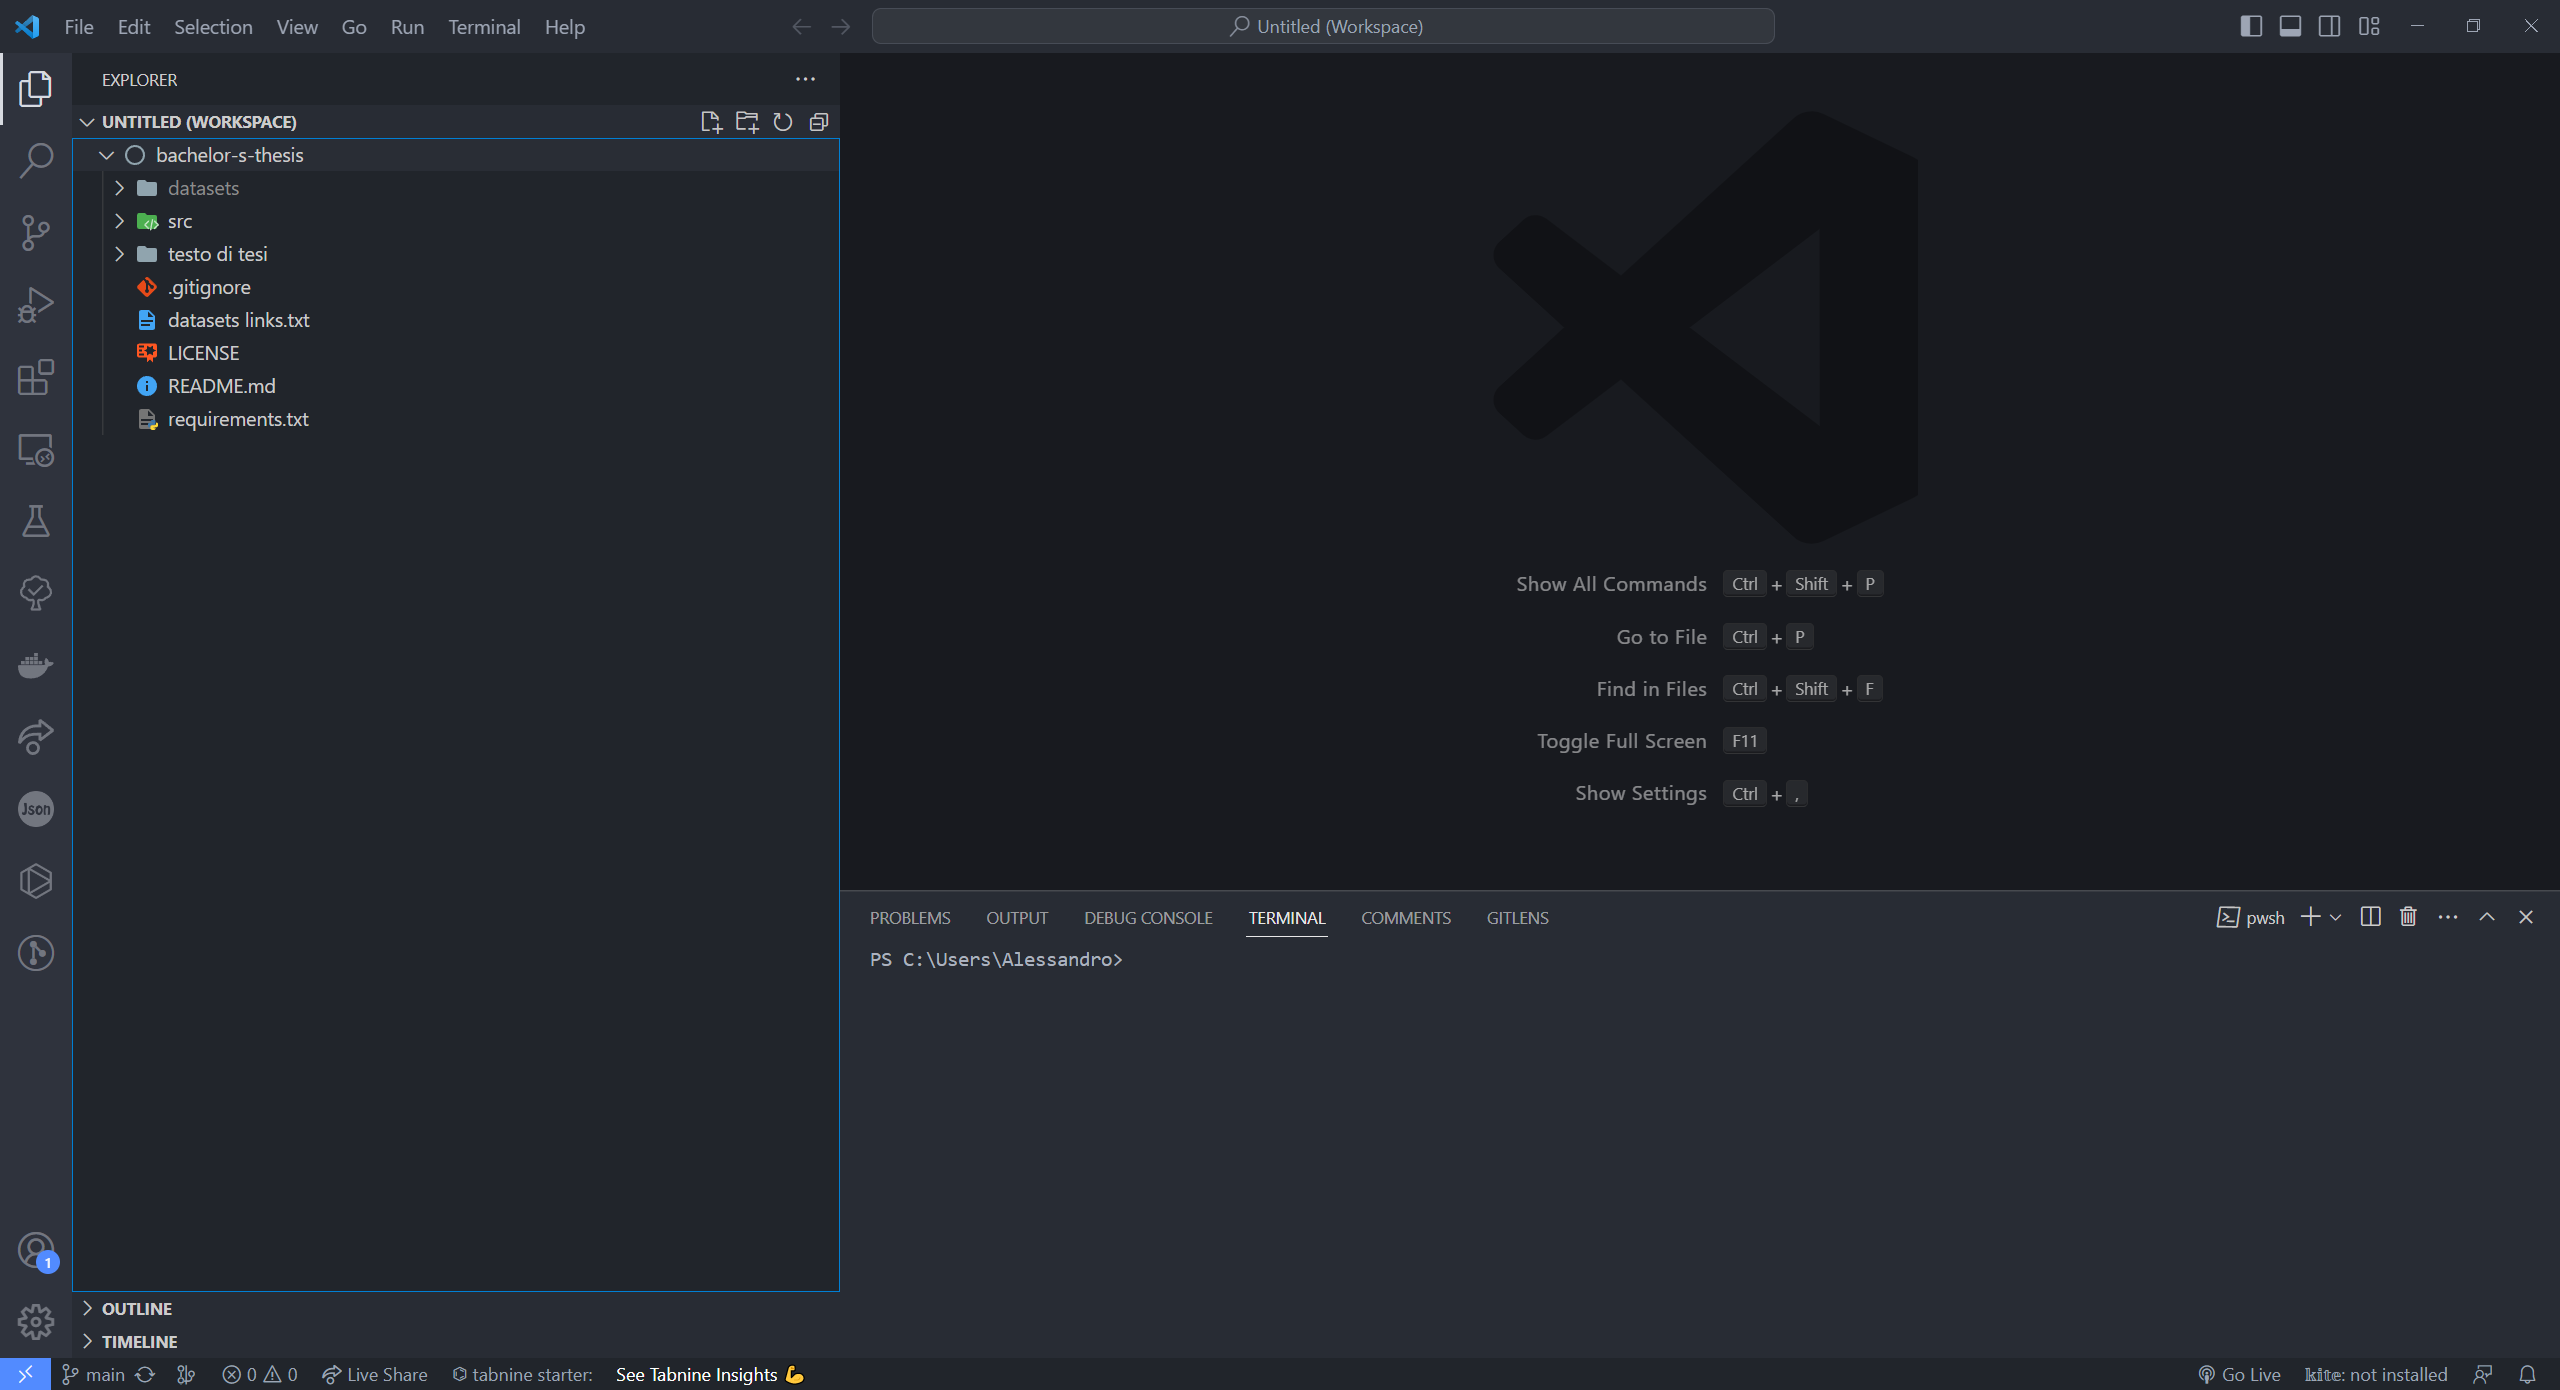
\includegraphics[width=0.72\linewidth]{images/image4.png}
        \caption{La cartella della repository è aperta all'interno di Visual Studio Code}
        \label{img:4}
    \end{center}
\end{figure}

\item Espandere le seguenti cartelle fino ad arrivare al file chiamato “interfaccia.py”, come visibile in \ref{img:5}
\begin{figure}
    \begin{center}    
        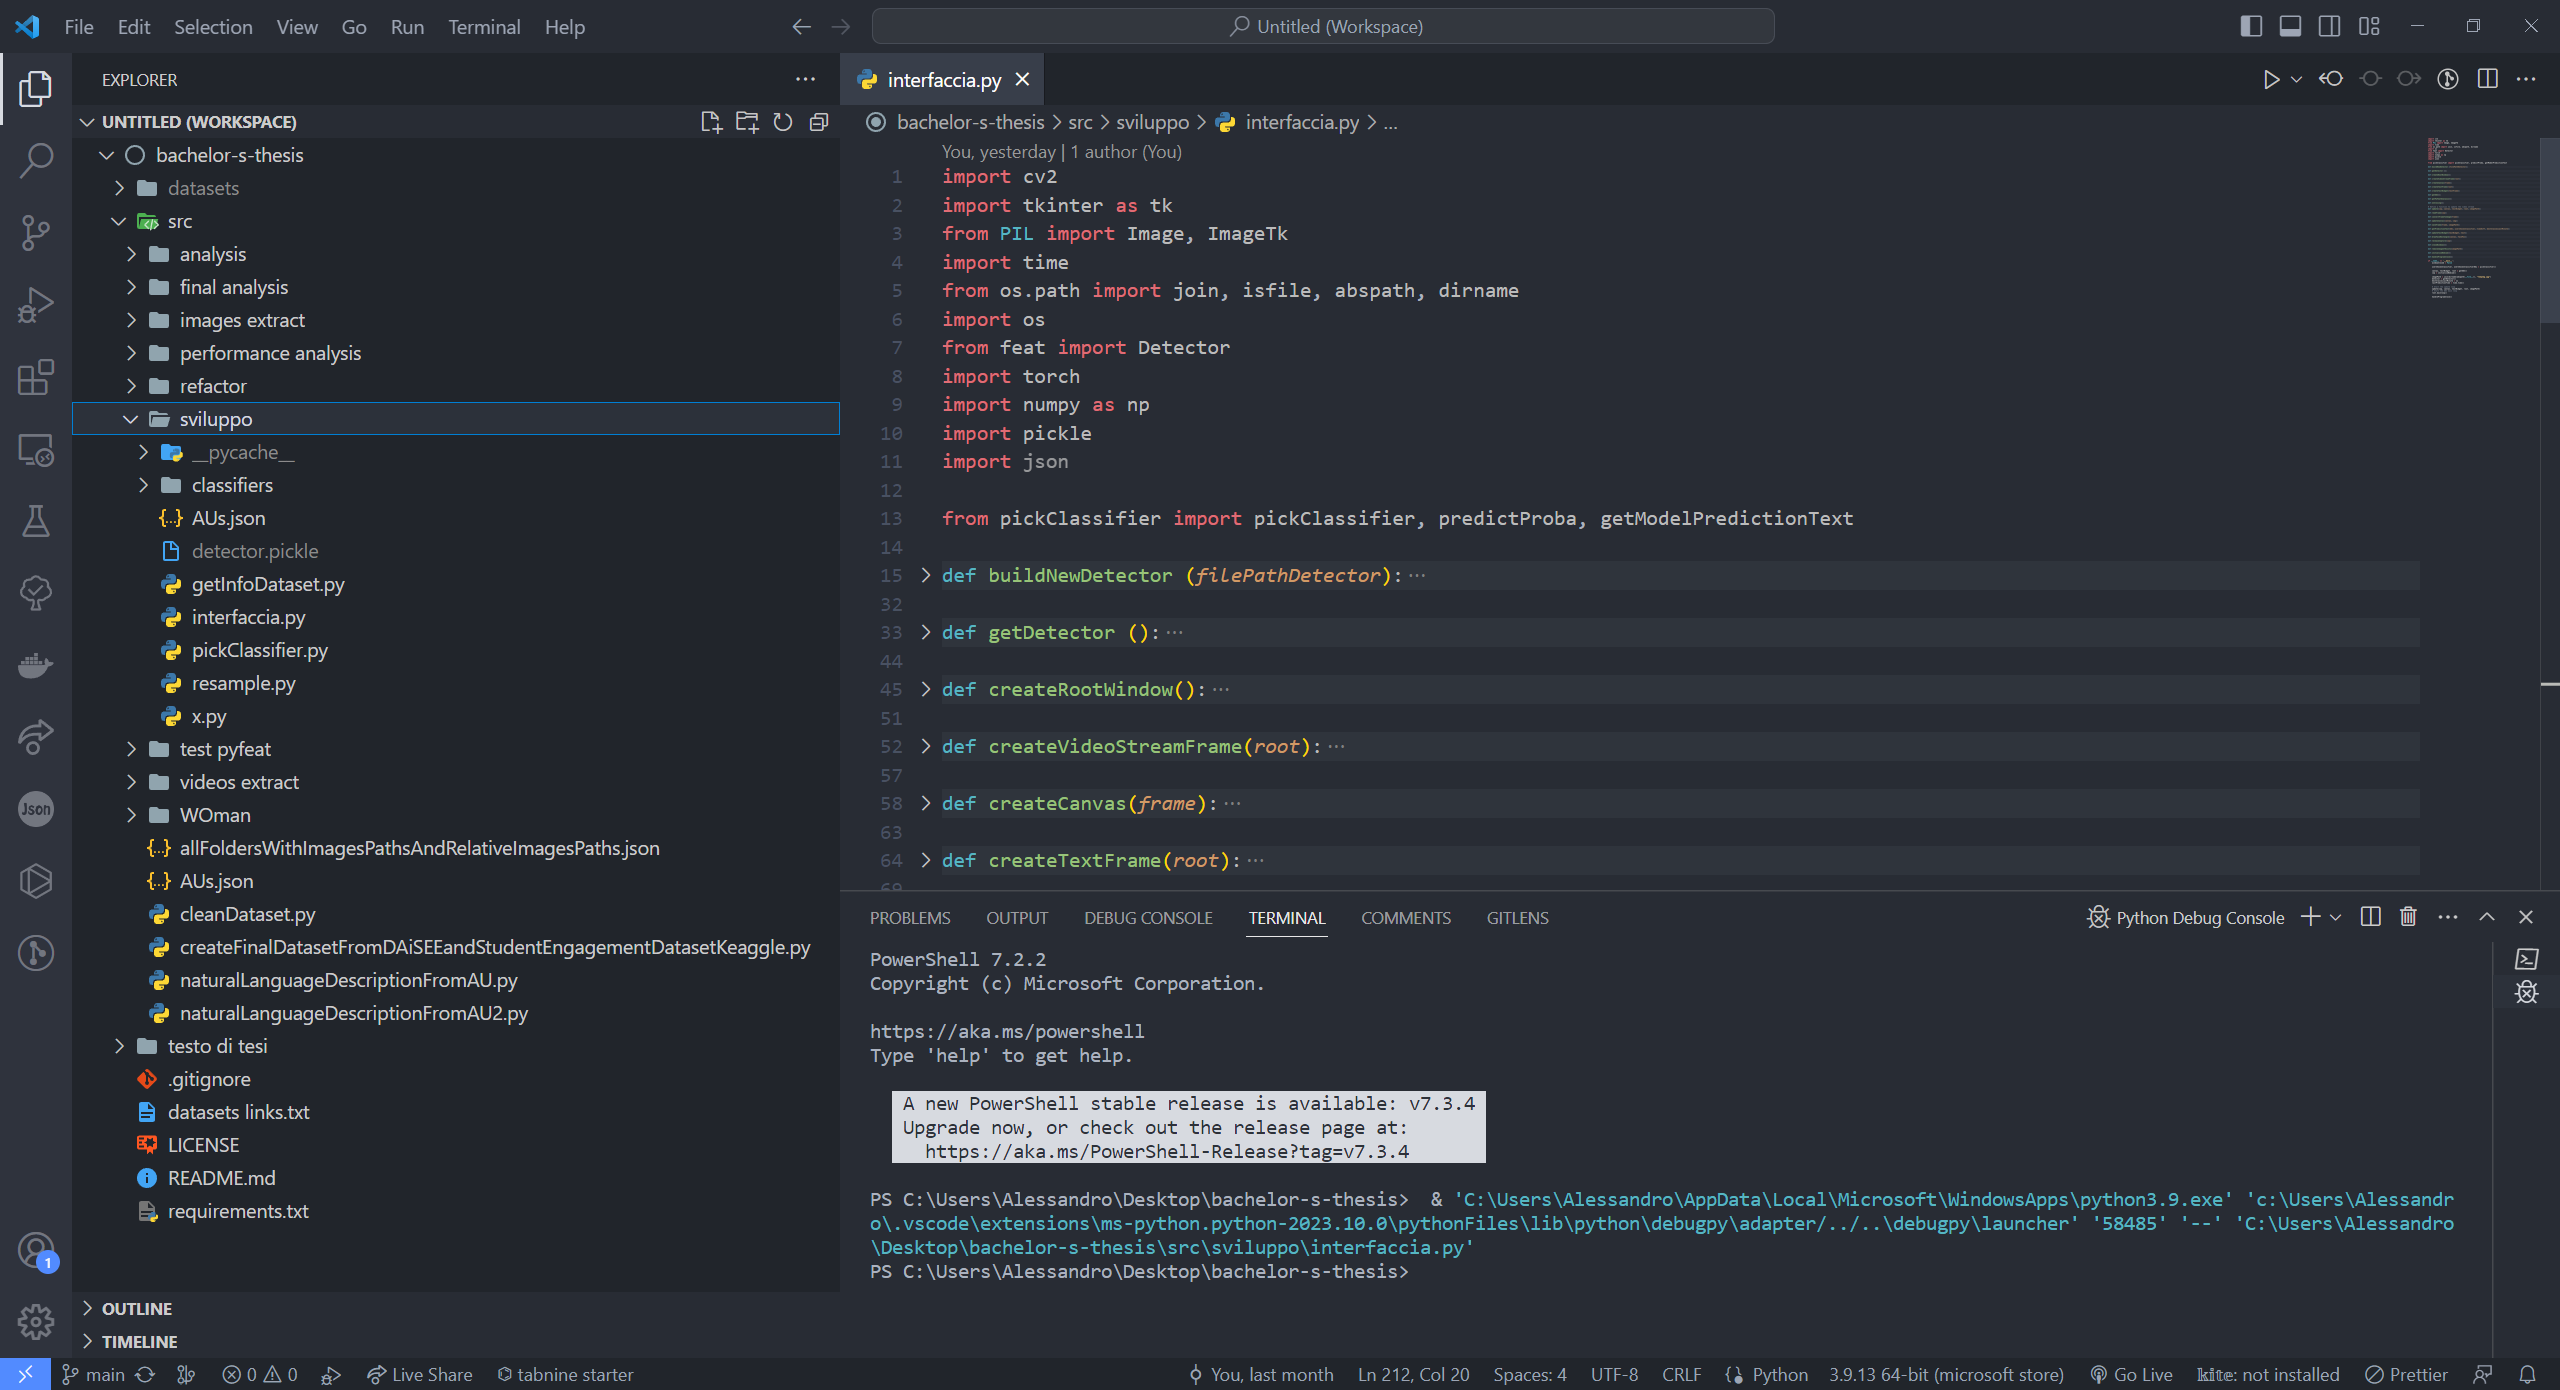
\includegraphics[width=0.72\linewidth]{images/image5.png}
        \caption{Apertura del file interfaccia.py}
        \label{img:5}
    \end{center}
\end{figure}
\newpage
\item Ora premere sull’icona di “Run and Debug” presente sulla sinistra e premere sul bottone “Run and Debug”, come visibile in \ref{img:6}
\begin{figure}
    \begin{center}    
        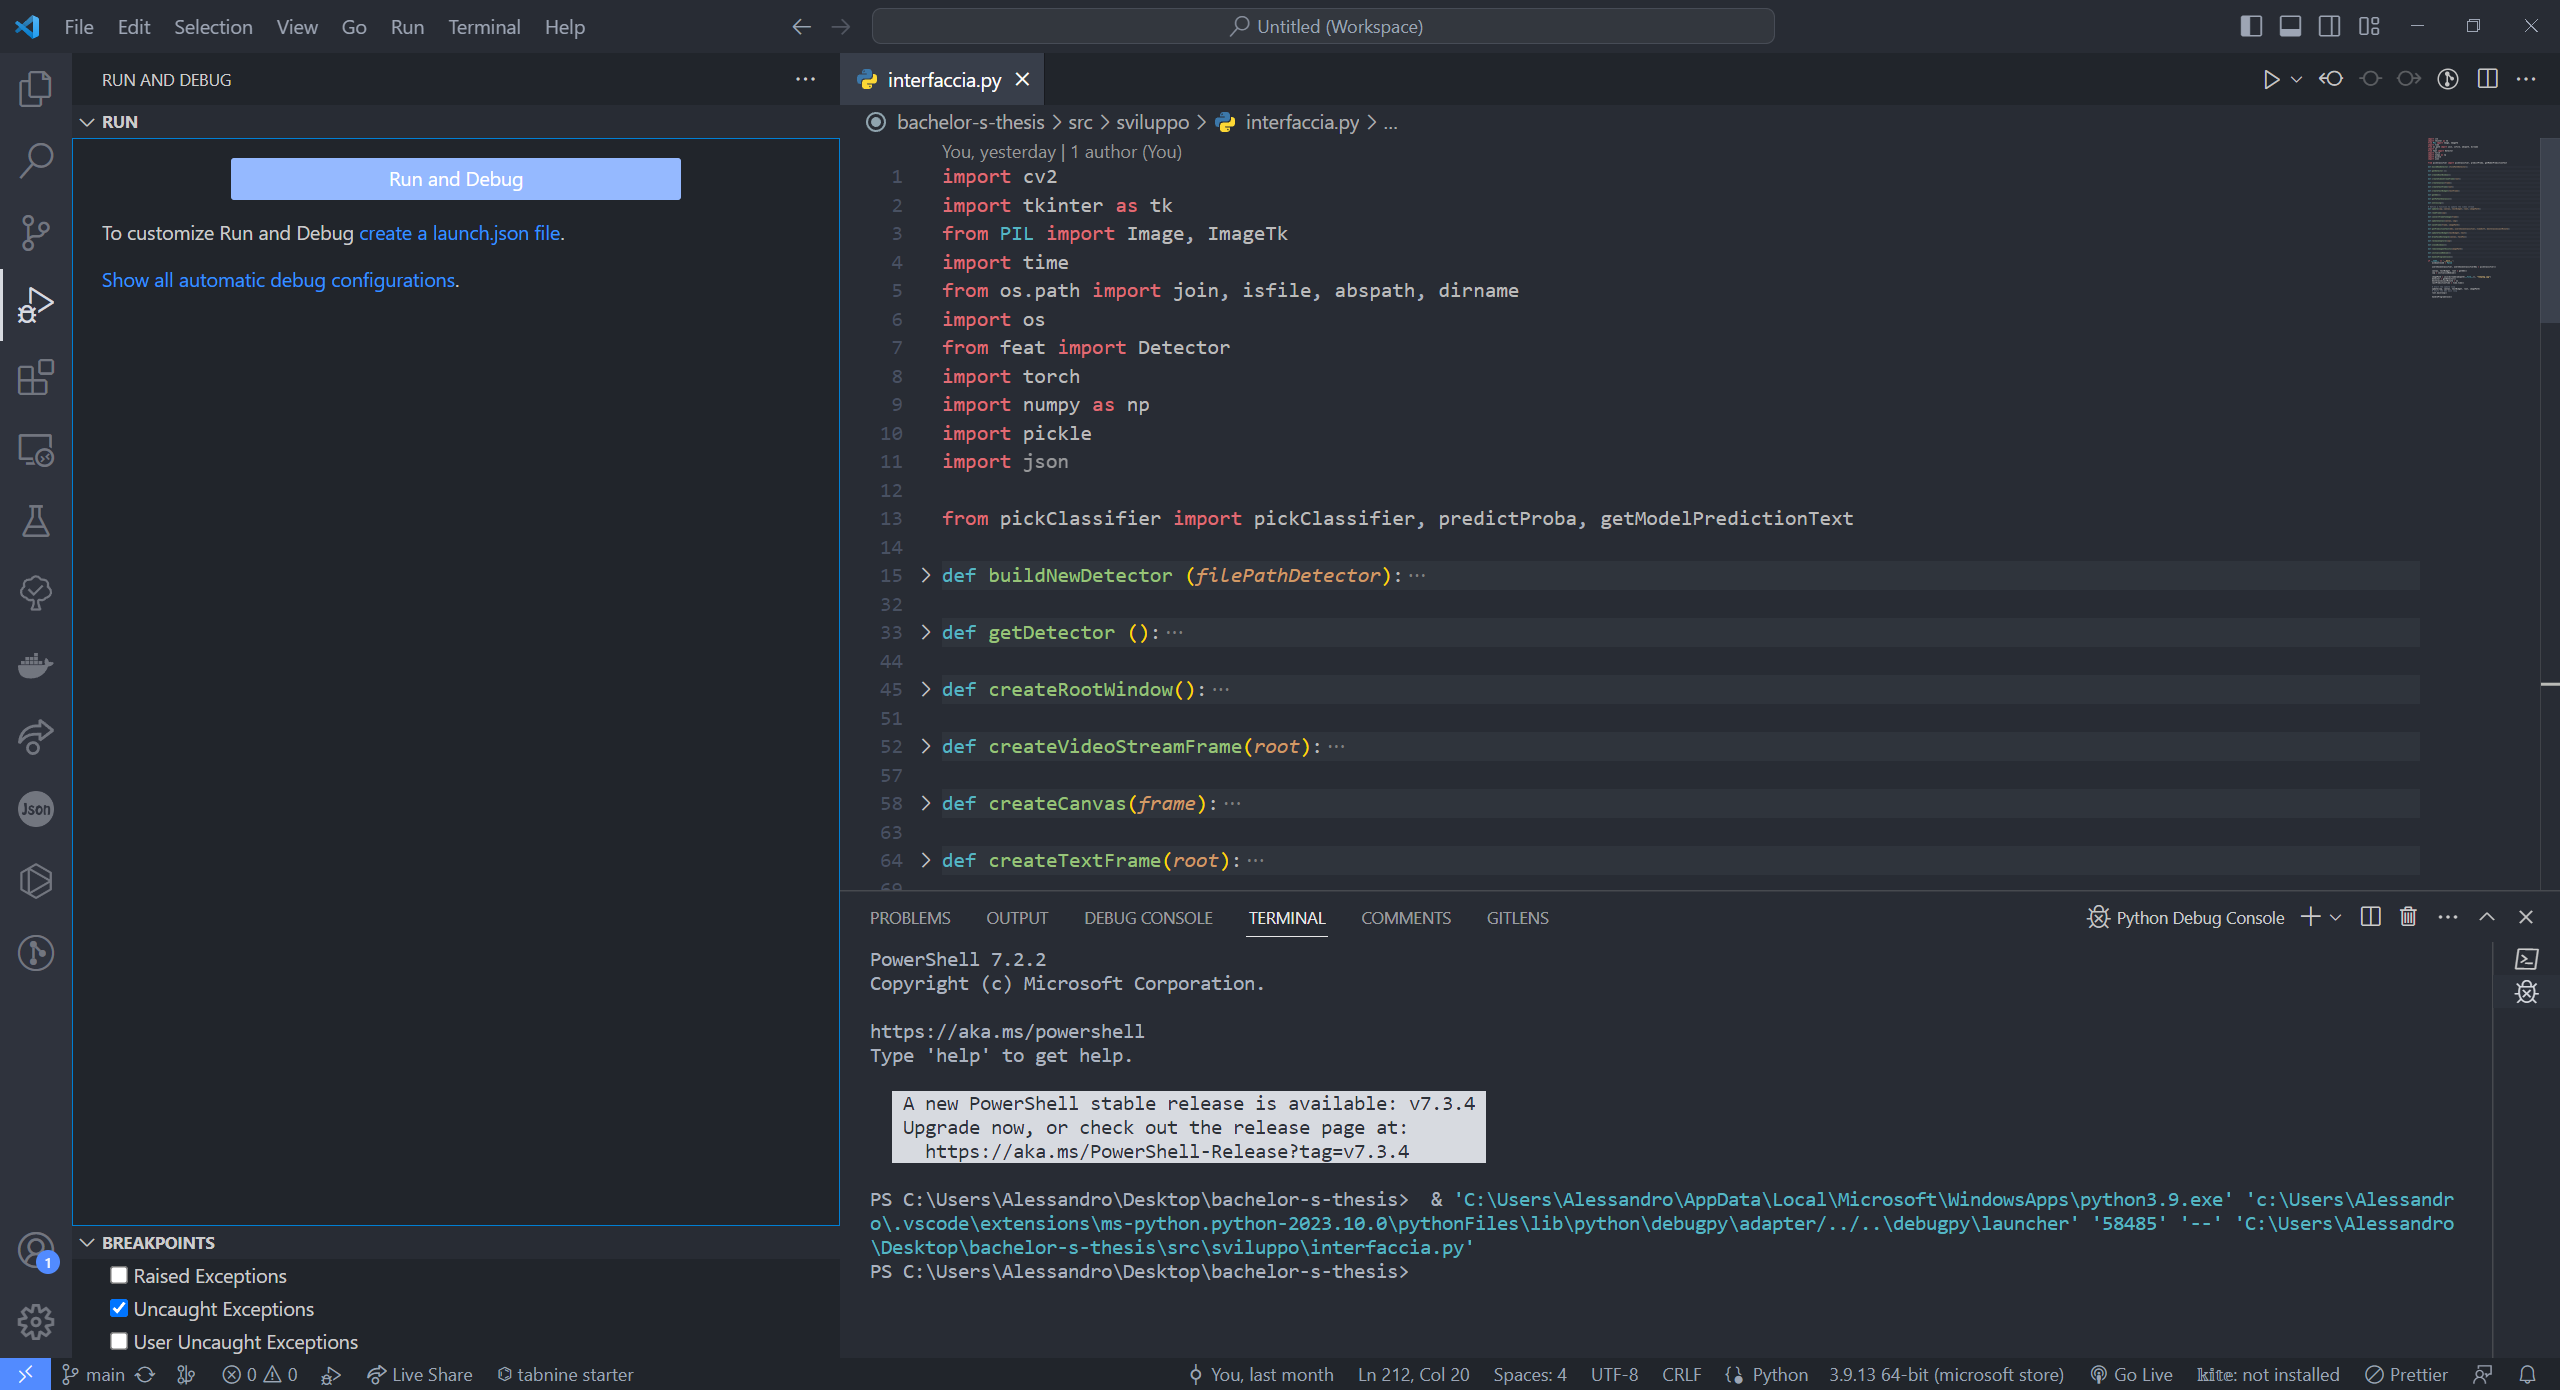
\includegraphics[width=0.72\linewidth]{images/image6.png}
        \caption{Run and Debug}
        \label{img:6}
    \end{center}
\end{figure}


\item Una volta premuto il bottone si presenterà questo menu dal quale si consiglia di scegliere la prima opzione, “Python File”, come visibile in \ref{img:7}
\begin{figure}
    \begin{center}    
        
\includegraphics[width=0.72\linewidth]{images/image7.png}
        \caption{Selezione "Python File"}
        \label{img:7}
    \end{center}
\end{figure}
\newpage
\item Ora il programma si avvierà e la prima schermata presente sarà quella visibile in \ref{img:8}
\begin{figure}
    \begin{center}    
        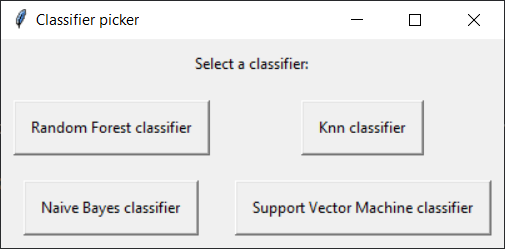
\includegraphics[width=0.72\linewidth]{images/image8.png}
        \caption{Prima schermata}
        \label{img:8}
    \end{center}
\end{figure}

da qui è possibile scegliere fra i 4 classificatori creati per il progetto, si consiglia di scegliere, premendo il relativo bottone, il “Random Forest classifier” in quanto risulta essere il più performante fra i quattro.
\item Una volta selezionato il classificatore si presenterà l’interfaccia finale dell’applicativo.
\end{itemize}

\section{Descrizione dell’interfaccia}
L’interfaccia presente è quella visibile in \ref{img:9}
\begin{figure}
    \begin{center}    
        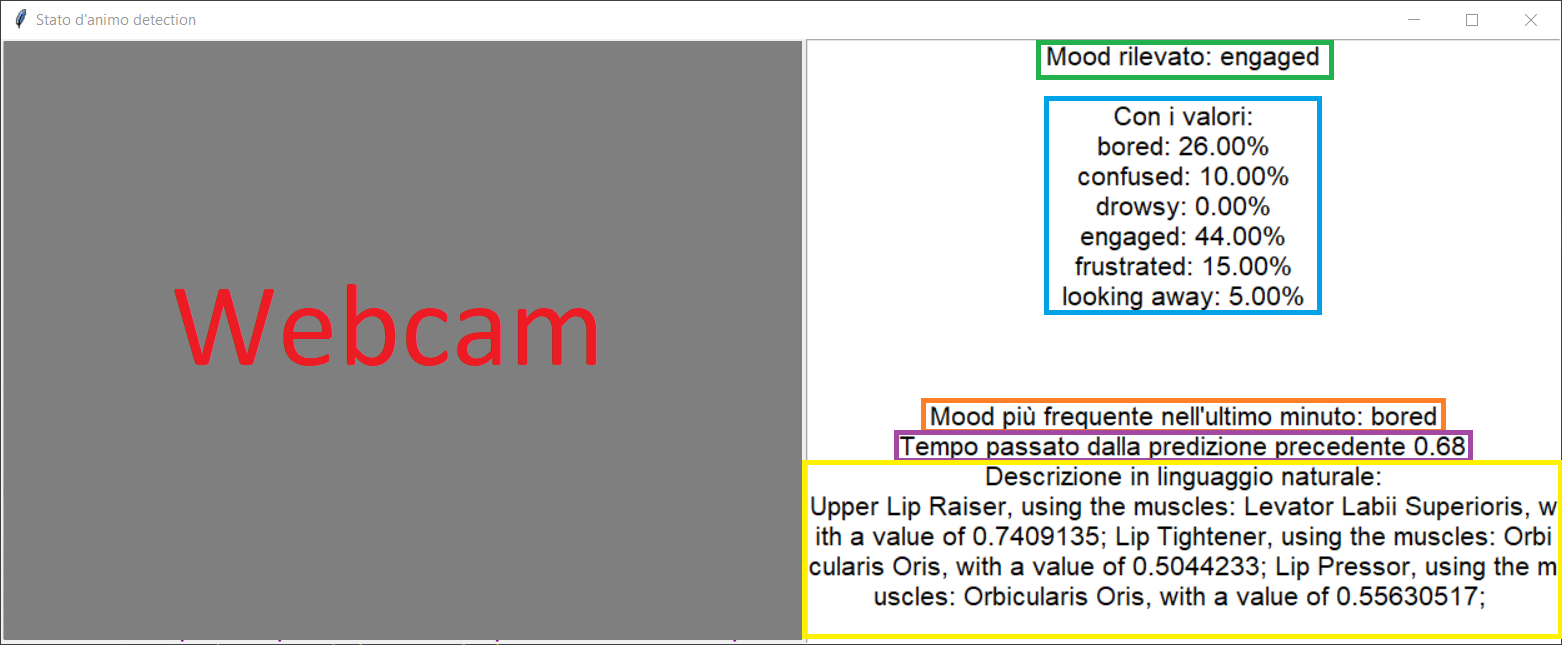
\includegraphics[width=0.72\linewidth]{images/image9.png}
        \caption{Schermata principale dell'interfaccia}
        \label{img:9}
    \end{center}
\end{figure}

\begin{itemize}
\item Nella metà a sinistra è presente lo stream della videocamera dalla quale vengono estratte le informazioni
\item nella sezione in verde è presente il mood rilevato nel frame letto nel momento della visualizzazione
\item nella sezione in blu è presente l’intera predizione effettuata dal modello predittivo (il mood mostrato nella sezione in verde è ovviamente il mood con il valore maggiore fra questi)
\item nella sezione in arancione è presente il mood che è stato più frequente nell’ultimo minuto in modo che si possa avere un’idea più precisa del mood della persona che sta utilizzando il sistema
\item nella sezione in viola è presente, in secondi, il tempo passato dalla predizione precedentemente effettuata, questo campo serve per effettuare una veloce valutazione delle performance del sitema sulla macchina
\item nella sezione in giallo è presente la descrizione in linguaggio naturale delle Action Units rilevate, questa si compone di:
\begin{itemize}
\item il nome associato all’action units che risulta attiva in quel momento.
\item il muscolo relativo contratto
\item il valore rilevato per l’Action Unit
\end{itemize}
Tutte le descrizioni delle action units sono presenti in sequenza separate da un punto e virgola.
\end{itemize}




\bibliographystyle{plain}  

\end{document}



